\chapter{Технологическая часть}

В данном разделе производится выбор средств реализации, приведятся требования к ПО, листинги реализованных алгоритмов решения задачи коммивояжера, а также результаты их тестированиия.

\section{Требования к ПО}

На вход программе подаются количество городов и симметричная матрица смежности, а также параметры $\alpha$ (коэффициент жадности), po (коэффициент испарения) и tmax (время жизни колонии) для муравьиного алгоритма. На выходе должны быть получены решения задачи коммивояжера, найденые с помощью каждого реализованного алгоритма: алгоритма полного перебора и муравьиного алгоритма. 

\section{Выбор средств реализации}

В качестве языка программирования для реализации данной лабораторной работы был выбран язык Python  \cite{PythonBook}. Он позволяет быстро реализовывать различные алгоритмы без выделения большого времени на проектирование сруктуры программы и выбор типов данных. 

Кроме того, в Python есть библиотека time, которая предоставляет функцию process\_time для замера процессорного времени \cite{process_time_text}.

В качестве среды разработки выбран PyCharm. Он является кросс-платформенным, а также предоставляет удобный и функциональнаый отладчик и средства для рефакторинга кода, что позволяет быстро находить и исправлять ошибки \cite{pycharm}.

\section{Листинги кода}

В листинге \ref{full} представлена реализация алгоритма полного перебора для решения задачи коммивояжера.

\clearpage
\begin{lstlisting}[caption=Алгоритм полного перебора,
	label={full}]
	def full_search(D, n_cities):
		min_way_length = INF
		min_way = None
		cur_way = []
		
		while next_set(cur_way, n_cities):
			cur_way_lenth = count_way_lenth(D, cur_way + [cur_way[0], ])
			if cur_way_lenth < min_way_length:
				min_way_length = cur_way_lenth
				min_way = cur_way
		
		return min_way_length, min_way + [min_way[0]]
\end{lstlisting}

\clearpage
В листинге \ref{ant} представлена реализация муравьиного алгоритма для решения задачи коммивояжера.


\begin{lstlisting}[caption=Муравьиный алгоритм,
	label={ant}]
	def ant_search(D, n_cities, alpha=ALPHA, po=PO, tmax=TMAX):
		Q = 0
		for i in range(n_cities):
			for j in range(i):
				if D[i][j] < INF:
					Q += D[i][j]
		beta = 1 - alpha
		
		eta = [[0 for i in range(n_cities)] for j in range(n_cities)]
		tau = [[0 for i in range(n_cities)] for j in range(n_cities)]
		for i in range(n_cities):
			for j in range(i):
				eta[i][j] = 1 / D[i][j]
				eta[j][i] = 1 / D[j][i]
				tau[i][j] = 2 * EPS
				tau[j][i] = 2 * EPS
		
		min_way_length = INF
		
	
		for t in range(tmax):
			visited_cities = [[i] for i in range(n_cities)]
		
			for k in range(n_cities):
		
				while len(visited_cities[k]) != n_cities:
					P_ch = [0 for i in range(n_cities)]
					for j in range(n_cities):
						if j not in visited_cities[k]:
							i = visited_cities[k][-1]
							P_ch[j] = (tau[i][j] ** alpha) * (eta[i][j] ** beta)
					
					P_zn = sum(P_ch)
					for j in range(n_cities):
						P_ch[j] /= P_zn
					
					coin = random()
					summ, j = 0, 0
					while summ < coin:
						summ += P_ch[j]
						j += 1
					visited_cities[k].append(j - 1)
				
				visited_cities[k].append(visited_cities[k][0])
				way_length = count_way_lenth(D, visited_cities[k])
				
			
				if way_length < min_way_length:
					min_way_length = way_length
					min_way = visited_cities[k]
			
		
			for i in range(n_cities):
				for j in range(i):
					delta_tau = 0
				
					for k in range(n_cities):
						way_length = count_way_lenth(D, visited_cities[k])
						for m in range(1, len(visited_cities[k])):
							if (visited_cities[k][m], visited_cities[k][m - 1]) in ((i, j), (j, i)):
								delta_tau += Q / way_length
								break
			
				tau[i][j] = tau[i][j] * (1 - po) + delta_tau
				if tau[i][j] < EPS:
					tau[i][j] = EPS
		
		return min_way_length, min_way
\end{lstlisting}

\clearpage
В листинге \ref{help} представлены реализации вспомогательных функций.


\begin{lstlisting}[caption=Вспомогательные функции,
	label={help}]

def next_set(a, n):
	if not a:
		for i in range(n):
			a.append(i)
		return True
	
	j = n - 2
	while j != -1 and a[j] > a[j + 1]:
		j -= 1
	if j == -1:
		return False  
	
	k = n - 1
	while a[j] > a[k]:
		k -= 1
	a[j], a[k] = a[k], a[j]
	
	l = j + 1
	r = n - 1
	while l < r:
		a[l], a[r] = a[r], a[l]
		l += 1
		r -= 1
	return True

def count_way_lenth(D, visited_cities):
	lk = 0
	for l in range(1, len(visited_cities)):
		i = visited_cities[l - 1]
		j = visited_cities[l]
		lk += D[i][j]
	
	return lk
\end{lstlisting}


\clearpage
\section{Тестирование}

На рисунке \ref{fig:work_example} приведен пример работы программы.


\begin{figure}[h!]
	
	\centering{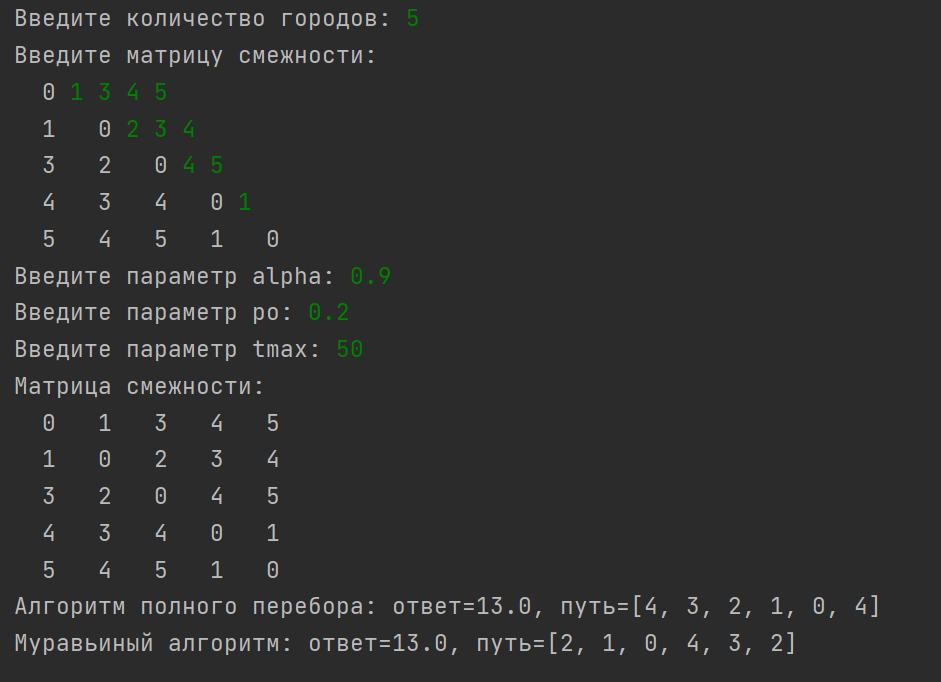
\includegraphics[scale=1]{inc/img/work_example.png}}
	
	\caption{Пример работы программы}
	
	\label{fig:work_example}
	
\end{figure}

\clearpage
В таблице ~\ref{tabular:test_rec} приведены функциональные тесты для алгоритмов решения задачи коммивояжера:алгоритма полного перебора и муравьиного алгоритма. Тест считается успешно пройденным, если длина найденного пути совпадает с ожидаемой, а в найденном пути созраняется ожидаемая последовательность городов (то есть город, с которого начинается посследовательность, не является принципиальным). Все тесты пройдены успешно каждым алгоритмом.

\begin{table}[h!]
	\begin{center}
		
		\caption{\label{tabular:test_rec} Тестирование функций}
		\begin{tabular}{c@{\hspace{7mm}}c@{\hspace{7mm}}c@{\hspace{7mm}}c@{\hspace{7mm}}}
			\hline
			Матрица смежности & Ожидаемый наименьший путь \\ \hline
			\vspace{4mm}
			$\begin{pmatrix}
				0 &  3 &  4 &  7\\
				3 &  0 &  3 &  7\\
				4 &  3 &  0 &  7\\
				7 &  7 &  7 &  0
			\end{pmatrix}$ &
			20, [0, 1, 2, 3, 0]\\
			\vspace{2mm}
			\vspace{2mm}
			$\begin{pmatrix}
				0 &  1 &  1 &  1 &  1 &  1\\
				1 &  0 &  1 &  1 &  1 &  1\\
				1 &  1 &  0 &  1 &  1 &  1\\
				1 &  1 &  1 &  0 &  1 &  1\\
				1 &  1 &  1 &  1 &  0 &  1\\
				1 &  1 &  1 &  1 &  1 &  0\\
			\end{pmatrix}$ &
			6, [0, 1, 2, 3, 4, 5, 0]\\
			\vspace{2mm}
			\vspace{2mm}
			$\begin{pmatrix}
				0 &  1 &  INF &  4\\
				1 &  0 &  2 &  INF\\
				INF &  2 &  0 &  3\\
				4 &  INF &  3 &  0
			\end{pmatrix}$ &
			10, [0, 1, 2, 3, 0]\\
		\end{tabular}
	\end{center}
\end{table}


\section*{Вывод}

Был производен выбор средств реализации, приведены требования к ПО, реализованы и протестированы алгоритмы регения задачи коммивояжера.
